\documentclass{article}
\usepackage[T1]{fontenc}
\usepackage{lmodern}
\usepackage[polish]{babel}
\usepackage{graphicx}
\usepackage{float}
\usepackage{hyperref}
\usepackage{amsmath}
\usepackage{listings}
\usepackage{xcolor}

\usepackage[a4paper, margin=2.54cm]{geometry}

\title{Praca domowa 4\\Sieci neuronowe}
\author{Damian Jankowski s188597}

\begin{document}

\maketitle

\section{Wstęp}

Celem pracy domowej było zapoznanie się z działaniem sieci neuronowych.
Zadaniem było zbudowanie sieci neuronowej, która będzie rozpoznawać czy dany
punkt jest wewnątrz jakiegoś obszaru czy na zewnątrz oraz porównanie
działania sieci neuronowej z gotowymi rozwiązaniami.


Wybrałem trapez opisany za pomocą tych czterech równań:
\begin{equation}
    \begin{cases}
        x_2 = -\frac{2}{3}x_1+4 \\
        x_2 = \frac{1}{2}x_1 \\
        x_2 = \frac{1}{2}x_1 + 3 \\
        x_2 = -\frac{3}{2}x_1 + 14
    \end{cases}
\end{equation}
\begin{figure}[H]
    \centering
    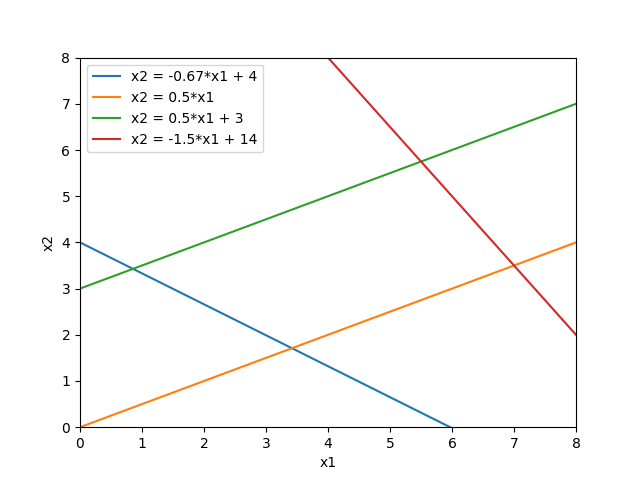
\includegraphics[width=0.6\textwidth]{trapez.png}
    \caption{Wykres trapezu wykorzystywanego do tego zadania}
\end{figure}

\section{Opis budowy sieci neuronowej}

Sieć składa się z 2 warstw. Pierwsza warstwa ma 4 neurony odpowiadające
czterem równaniom, które opisują trapez. Druga warstwa ma jeden neuron, który
ma za zadanie zwrócić 1 jeśli punkt jest wewnątrz trapezu lub 0 jeśli punkt
jest na zewnątrz.

Pojedynczy neuron można opisać równaniem:
\begin{equation}
    \sigma(w_1x_1 + w_2x_2 + w_3)
\end{equation}
gdzie $w_i$ to wagi, $x_i$ to wejścia, a $\sigma$ to funkcja
aktywacji. 

W tym przypadku jako funkcję aktywacji użyłem funkcji stepu:
\begin{equation}
    \sigma(x) = \begin{cases}
        1 & \text{dla } x > 0 \\
        0 & \text{dla } x \leq 0
    \end{cases}
\end{equation}

Dla tego zadania kolejne neurony są opisane następującymi równaniami:

\begin{enumerate}
    \centering
    \item $\frac{2}{3}x_1 + x_2 - 4 = 0$
    \item $-\frac{1}{2}x_1 + x_2 = 0$
    \item $\frac{1}{2}x_1 - x_2 + 3 = 0$
    \item $-\frac{3}{2}x_1 - x_2 + 14 = 0$
\end{enumerate}

Piąty neuron jest opisany równaniem:
\begin{equation}
    \sigma(w_1N_1 + w_2N_2 + w_3N_3 + w_4N_4 - w_5\cdot1)
\end{equation}
gdzie $N_i$ to wyjścia z neuronów pierwszej warstwy, a $w_i$ to wagi.

Wagi zostały dobrane w taki sposób, by każdy neuron pierwszej warstwy zwracał
1, gdy punkt znajduje się po poprawnej stronie prostej. Wyglądają następująco:
\begin{equation}
    w_1 = w_2 = w_3 = w_4 = 1 \quad w_5 = -3
\end{equation}

Waga biasa została ustawiona jako -3, ponieważ gdy wszystkie neurony
pierwszej warstwy zwrócą 1 (punkt znajduje się wewnątrz trapezu), to piąty
neuron również zwróci 1. W każdym innym przypadku zwróci 0.

\begin{figure}[H]
    \centering
    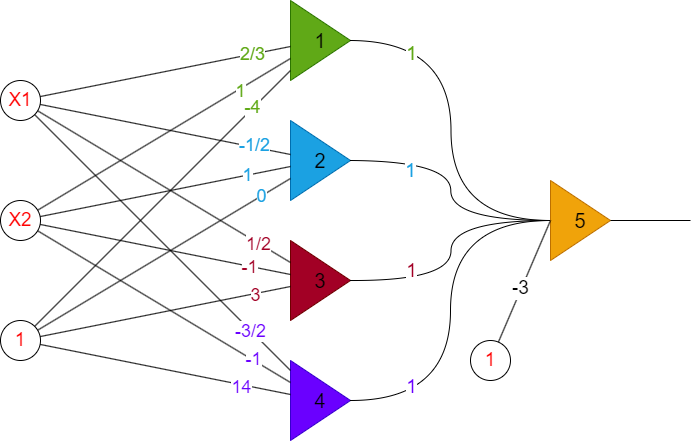
\includegraphics[width=0.9\textwidth]{sieć.png}
    \caption{Schemat sieci neuronowej}
\end{figure}

\newpage

\section{Zasada działania modelu}

Zasadę działania modelu można opisać następująco dla przykładowcych punktów:

\begin{itemize}
    \centering
    \item $P_1 = (4, 3)$
    \item $P_2 = (7, 2)$
\end{itemize}
Dla punktu $P_1$ neurony zwracają następujące wartości:
\begin{itemize}
    \centering
    \item $N_1 = \sigma(\frac{2}{3}\cdot4 + 3 - 4) = 1$
    \item $N_2 = \sigma(-\frac{1}{2}\cdot4 + 3) = 1$
    \item $N_3 = \sigma(\frac{1}{2}\cdot4 - 3 + 3) = 1$
    \item $N_4 = \sigma(-\frac{3}{2}\cdot4 - 3 + 14) = 1$
    \item $N_5 = \sigma(1 + 1 + 1 + 1 - 3) = 1$
\end{itemize}
Według tej sieci punkt $P_1$ znajduje się wewnątrz trapezu.

Natomiast dla punktu $P_2$:
\begin{itemize}
    \centering
    \item $N_1 = \sigma(\frac{2}{3}\cdot7 + 2 - 4) = 1$
    \item $N_2 = \sigma(-\frac{1}{2}\cdot7 + 2) = 0$
    \item $N_3 = \sigma(\frac{1}{2}\cdot7 - 2 + 3) = 1$
    \item $N_4 = \sigma(-\frac{3}{2}\cdot7 - 2 + 14) = 1$
    \item $N_5 = \sigma(1 + 0 + 1 + 1 - 3) = 0$
\end{itemize}
Według tej sieci punkt $P_2$ znajduje się na zewnątrz trapezu.

\section{Test modelu teoretycznego}

Do przetestowania modelu teoretycznego, wykorzystałem bibliotekę
\textit{keras}. Wylosowałem 1000 punktów z przedziału $[0, 8]$ i
przetestowałem je na sieci, której wagi są wyznaczone przez
równania prostych. Wyniki przedstawia poniższy wykres:

\begin{figure}[H]
    \centering
    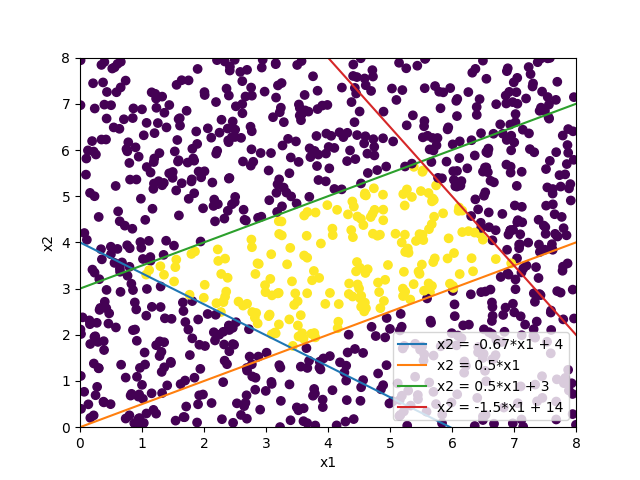
\includegraphics[width=0.6\textwidth]{punkty_teor.png}
    \caption{Wykres punktów z zaznaczoną predykcją dla modelu teoretycznego}
\end{figure}

\section{Porównanie modelu teoretycznego z gotowym modelem}

Do porównania modelu teoretycznego z gotowym modelem wykorzystałem
ponownie bibliotekę \textit{keras}. Ponownie również wylosowałem
1000 punktów z przedziału $[0, 8]$, które służyły do trenowania modelu.

Jako funkcję aktywacji wybrałem funkcję \textit{sigmoid}, natomiast
jako funkcję straty wybrałem \textit{mse}. Struktura sieci jest identyczna
jak w modelu teoretycznym. Ilość epok wynosi 100.

\begin{figure}[H]
    \centering
    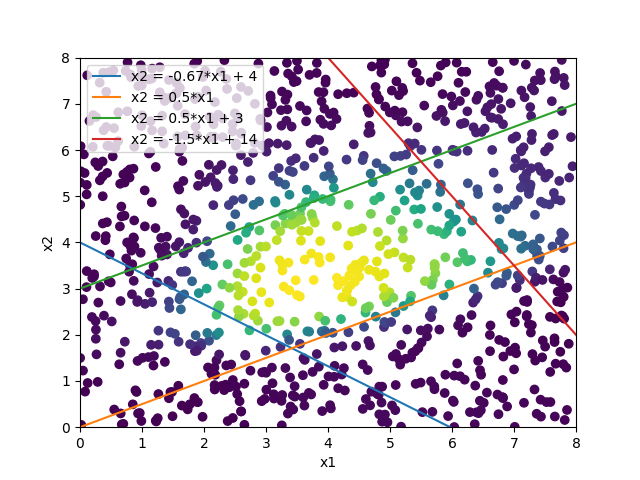
\includegraphics[width=0.6\textwidth]{punkty.png}
    \caption{Wykres punktów testowych z zaznaczoną predykcją dla gotowego modelu}
\end{figure}


Dla warstwy pierwszej:

Model zdecydował o wybraniu następujących wag:
\begin{equation*}
    \begin{bmatrix}
        w_{11} & w_{21} & w_{31} & w_{41} \\
        w_{12} & w_{22} & w_{32} & w_{42} \\
    \end{bmatrix}
    =
    \begin{bmatrix}
        0.6038228  & 2.0212314 &  0.9918629 & -1.7553812 \\
        0.79492724 & -2.2487426 & -3.4824367 & -0.0563702 \\
    \end{bmatrix}
\end{equation*}

Oraz następujących wag biasa:
\begin{equation*}
    \begin{bmatrix}
        w_{13} & w_{23} & w_{33} & w_{43}
    \end{bmatrix}
    =
    \begin{bmatrix}
        -6.95771  &  4.133127 &  3.4448078 & 3.7257853
    \end{bmatrix}
\end{equation*}

Natomiast dla drugiej warstwy:

Model zdecydował o wybraniu następujących wag:
\begin{equation*}
    \begin{bmatrix}
        w_{51} \\
        w_{52} \\
        w_{53} \\
        w_{54} \\
    \end{bmatrix}
    =
    \begin{bmatrix}
        -6.9642315 \\
         2.9435923 \\
        -7.6793256 \\
        -5.9134836 \\
    \end{bmatrix}
\end{equation*}

Oraz następujących wag biasa:
\begin{equation*}
    \begin{bmatrix}
        w_{55}
    \end{bmatrix}
    =
    \begin{bmatrix}
        0.9833915
    \end{bmatrix}
\end{equation*}

Dokładność modelu wynosła $95.70 \% $, natomiast funkcja straty
wyniosła $0.0385$.

\section{Wnioski}

Jak widać na wykresach, oba modele dobrze radzą sobie z klasyfikacją,
jednakże model teoretyczny jest bardziej dokładny. Wynika to z faktu,
że model teoretyczny korzysta już ze znanych równań prostych, natomiast
model gotowy musi nauczyć się tych równań samodzielnie. 

Ważnym czynnikiem w przypadku modelu gotowego jest również wybór odpowiedniej
funkcji aktywacji oraz funkcji straty, jak również ilość epok, które 
znacząco wpływają na dokładność modelu.




\section{Kod programu}
\lstinputlisting[
language=python,  
basicstyle=\small\tt,
keywordstyle=\color{blue},
backgroundcolor=\color{cyan!10}
]{main.py}

\end{document}